\documentclass[10pt,a4paper]{article}
\usepackage[margin=2cm]{geometry}
\usepackage[T1]{fontenc}
\usepackage{lmodern}
\usepackage{amsmath,amssymb,booktabs,multirow,colortbl}
\usepackage[table]{xcolor}
\usepackage{pgfplots}
\pgfplotsset{compat=1.18}
\usepackage{float}
\usepackage[hidelinks]{hyperref}
\usepackage{titlesec,enumitem}
\titleformat{\section}{\large\bfseries}{\thesection}{0.6em}{}
\titleformat{\subsection}{\normalsize\bfseries}{\thesubsection}{0.5em}{}
\setlist{itemsep=1pt,topsep=3pt}

\definecolor{cmag}{HTML}{1F6F8B}
\definecolor{cfis}{HTML}{6A8F3A}
\definecolor{cgrad}{HTML}{C0612B}
\definecolor{ctier}{HTML}{7B3F98}
\definecolor{crand}{HTML}{8A939C}
\newcommand{\gain}[1]{\textcolor{cmag}{\textbf{#1}}}
\pgfplotsset{
  accplot/.style={width=0.49\textwidth,height=5.6cm,grid=major,grid style={gray!20},
    tick label style={font=\scriptsize},label style={font=\footnotesize},title style={font=\small\bfseries},
    legend style={font=\scriptsize,draw=none,fill=white,fill opacity=0.85,text opacity=1},
    legend cell align=left,mark size=1.3pt},
  pslc/.style={black,densely dotted,thick,mark=square*,mark options={solid}},
  pslcmap/.style={black,thick,mark=square*},
  pgrad/.style={cgrad,thick,mark=*},
  pmag/.style={cmag,very thick,mark=*},
  pfis/.style={cfis,thick,dashed,mark=diamond*,mark options={solid}},
  phyb/.style={crand,thick,mark=o},
  pmap/.style={cmag,very thick,mark=*},
  pjoint/.style={cfis,thick,dashed,mark=diamond*,mark options={solid}},
  pnf/.style={cgrad,thick,mark=triangle*},
  ptier/.style={ctier,very thick,mark=*}}

\begin{document}

\begin{center}
{\LARGE\bfseries Contribution Results}\\[4pt]
{\large Reliable Hybrid SLC/MLC ReRAM Crossbars for Transformers}\\[4pt]
Shivansh Mittal, Sarvesh Joshi, Thumati Naveen Chandra Chowdary, Aryan Chakravorty\\
CS5290 Memory-Centric Computer Architecture, Indian Institute of Technology Guwahati
\end{center}

\section*{Step 1: What is compared}
The baseline is the HyFlexPIM hybrid (SVD components ranked by the loss gradient, 20\% in SLC) with the
all-SLC and all-MLC chips as references; it is documented in the separate \emph{Baseline Results}. Our four
contributions are evaluated with the same cell-level simulator on BERT-Base and DistilBERT (SST-2) and, for
contributions 1 and 2, on MNLI:
\begin{enumerate}
\item \textbf{Magnitude placement}: rank components by singular value $|\sigma_r|$ instead of the gradient.
\item \textbf{Fault-aware mapping}: after a chip is tested, place each component in the slot whose stuck
cells hurt it least (Fisher-weighted Hungarian assignment), using the free order of SVD components.
\item \textbf{Tier-aware training}: fine-tune on a freshly simulated chip at every step, each component under
the errors of the tier (SLC or MLC) it will be stored in.
\item \textbf{Generalisation to MNLI} of contributions 1 and 2.
\end{enumerate}
All placements, mappings and trained models are evaluated on the same simulated chips (same seeds), so
differences within an experiment are paired and given as mean $\pm$ standard error over chips. The hybrid chip
uses 9.2 cells per weight, 34\% fewer than all-SLC (14).

\section*{Step 2: The baseline's gaps}
The baseline document shows three gaps, which the contributions address in turn: (i) the HyFlexPIM gradient
placement falls behind all-SLC at high programming noise; (ii) stuck cells break every baseline, all-MLC at
0.1\% and the HyFlexPIM hybrid near chance at 1\%; (iii) even all-SLC loses 14--27 points at 1\% stuck cells.

\section*{Step 3: Contribution 1, magnitude placement}
\begin{figure}[H]
\centering
\begin{tikzpicture}
\begin{axis}[accplot,title={BERT-Base},xlabel={Programming noise $\sigma$ (\% of $G_{\max}$)},ylabel={Accuracy (\%)},
  xtick={0,1,2,3,5,7.5,10},ymin=60,ymax=92,legend pos=south west]
\addplot[pslc] table[x=x,y=all_slc]{data/noise_bert.dat}; \addlegendentry{All SLC}
\addplot[pmag] table[x=x,y=magnitude]{data/noise_bert.dat}; \addlegendentry{Magnitude (ours)}
\addplot[pfis] table[x=x,y=fisher]{data/noise_bert.dat}; \addlegendentry{Fisher (ours)}
\addplot[pgrad] table[x=x,y=gradient]{data/noise_bert.dat}; \addlegendentry{HyFlexPIM gradient}
\end{axis}
\end{tikzpicture}\hfill
\begin{tikzpicture}
\begin{axis}[accplot,title={DistilBERT},xlabel={Programming noise $\sigma$ (\% of $G_{\max}$)},
  xtick={0,1,2,3,5,7.5,10},ymin=60,ymax=92]
\addplot[pslc] table[x=x,y=all_slc]{data/noise_distil.dat};
\addplot[pmag] table[x=x,y=magnitude]{data/noise_distil.dat};
\addplot[pfis] table[x=x,y=fisher]{data/noise_distil.dat};
\addplot[pgrad] table[x=x,y=gradient]{data/noise_distil.dat};
\end{axis}
\end{tikzpicture}
\caption{Accuracy against programming noise, 20\% SLC, mean of 5 chips.}
\end{figure}

\begin{figure}[H]
\centering
\begin{tikzpicture}
\begin{axis}[accplot,title={BERT-Base, $\sigma=7.5\%$},xlabel={Share of components in SLC (\%)},ylabel={Accuracy (\%)},
  xtick={0,10,20,30,50,100},ymin=50,ymax=90,legend pos=south east]
\addplot[pmag] table[x=x,y=magnitude]{data/share_bert_075.dat}; \addlegendentry{Magnitude (ours)}
\addplot[pfis] table[x=x,y=fisher]{data/share_bert_075.dat}; \addlegendentry{Fisher (ours)}
\addplot[pgrad] table[x=x,y=gradient]{data/share_bert_075.dat}; \addlegendentry{HyFlexPIM gradient}
\end{axis}
\end{tikzpicture}\hfill
\begin{tikzpicture}
\begin{axis}[accplot,title={DistilBERT, $\sigma=7.5\%$},xlabel={Share of components in SLC (\%)},
  xtick={0,10,20,30,50,100},ymin=50,ymax=90]
\addplot[pmag] table[x=x,y=magnitude]{data/share_distil_075.dat};
\addplot[pfis] table[x=x,y=fisher]{data/share_distil_075.dat};
\addplot[pgrad] table[x=x,y=gradient]{data/share_distil_075.dat};
\end{axis}
\end{tikzpicture}
\caption{Accuracy against the share of components in SLC at $\sigma=7.5\%$, mean of 20 chips; 0\% is all-MLC,
100\% all-SLC.}
\end{figure}

\begin{table}[H]
\centering\small
\caption{Paired difference to magnitude, in correctly classified sentences out of 872 (mean $\pm$ standard
error; 100 chips per noise level, 300 overall, all SLC shares).}\label{t:paired}
\begin{tabular}{@{}llrrrr@{}}
\toprule
Model & Placement & $\sigma=3\%$ & 5\% & 7.5\% & All \\
\midrule
\multirow{2}{*}{BERT-Base} & Fisher & $-0.1\pm0.5$ & $-0.1\pm0.7$ & $+1.4\pm1.9$ & $+0.4\pm0.7$ \\
 & HyFlexPIM gradient & $-1.2\pm0.7$ & $-10.4\pm1.6$ & $-40.4\pm5.0$ & $-17.3\pm2.0$ \\
\midrule
\multirow{2}{*}{DistilBERT} & Fisher & $-0.4\pm0.7$ & $-1.3\pm0.7$ & $+0.0\pm1.7$ & $-0.6\pm0.7$ \\
 & HyFlexPIM gradient & $-0.9\pm0.7$ & $-4.0\pm1.0$ & $-18.4\pm2.6$ & $-7.8\pm1.1$ \\
\bottomrule
\end{tabular}
\end{table}

\begin{table}[H]
\centering\small
\caption{Smallest SLC share within half a point of all-SLC (shares tested: 5, 10, 20, 30, 50\%), and the
resulting cells per weight relative to all-SLC.}\label{t:need}
\begin{tabular}{@{}llccc@{}}
\toprule
Model & Placement & $\sigma=3\%$ & $\sigma=5\%$ & $\sigma=7.5\%$ \\
\midrule
\multirow{2}{*}{BERT-Base} & Magnitude (ours) & \gain{5\%} (59\% of cells) & \gain{5\%} (59\%) & \gain{30\%} (70\%) \\
 & HyFlexPIM gradient & 5\% (59\%) & 10\% (61\%) & not reached at 50\% \\
\midrule
\multirow{2}{*}{DistilBERT} & Magnitude (ours) & 5\% (59\%) & \gain{10\%} (61\%) & \gain{50\%} (79\%) \\
 & HyFlexPIM gradient & 5\% (59\%) & 20\% (66\%) & not reached at 50\% \\
\bottomrule
\end{tabular}
\end{table}

\noindent\textbf{Analysis.}
\begin{itemize}
\item Magnitude and Fisher are statistically indistinguishable at every noise level, while the HyFlexPIM
gradient falls further behind as noise grows (Table~\ref{t:paired}); at 5\% SLC and $\sigma=7.5\%$ the gap on
BERT-Base is $11.9\pm1.7$ points.
\item \textbf{Why.} Each crossbar column has its own 8-bit scale, and the column of component $r$ holds
$\sigma_r v_r$, so the weight error a fixed cell noise causes is proportional to $|\sigma_r|$. The Fisher score
multiplies this error size by the loss sensitivity; that it selects the same components as magnitude
suggests the error size dominates. The gradient measures sensitivity alone and misses it.
\item \textbf{Cost.} Magnitude needs half the SLC share of the gradient at $\sigma=5\%$ and is the only score
that reaches all-SLC at $\sigma=7.5\%$ (Table~\ref{t:need}). It needs no data or gradients.
\end{itemize}

\section*{Step 4: Contribution 2, fault-aware mapping}
\begin{figure}[H]
\centering
\begin{tikzpicture}
\begin{axis}[accplot,title={BERT-Base},xlabel={Stuck cells $p$ (\% of cells)},ylabel={Accuracy (\%)},
  symbolic x coords={0.2,0.5,1,2},xtick=data,ymin=45,ymax=93,legend pos=south west]
\addplot[pslc] table[x=x,y=slc]{data/recover_bert.dat}; \addlegendentry{All SLC}
\addplot[pslcmap] table[x=x,y=slc_map]{data/recover_bert.dat}; \addlegendentry{All SLC + mapping}
\addplot[phyb] table[x=x,y=hyb]{data/recover_bert.dat}; \addlegendentry{Hybrid, no mitigation}
\addplot[pmap] table[x=x,y=hyb_map]{data/recover_bert.dat}; \addlegendentry{Hybrid + fault-aware mapping}
\addplot[pjoint] table[x=x,y=joint]{data/recover_bert.dat}; \addlegendentry{Hybrid + joint mapping}
\end{axis}
\end{tikzpicture}\hfill
\begin{tikzpicture}
\begin{axis}[accplot,title={DistilBERT},xlabel={Stuck cells $p$ (\% of cells)},
  symbolic x coords={0.2,0.5,1,2},xtick=data,ymin=45,ymax=93]
\addplot[pslc] table[x=x,y=slc]{data/recover_distil.dat};
\addplot[pslcmap] table[x=x,y=slc_map]{data/recover_distil.dat};
\addplot[phyb] table[x=x,y=hyb]{data/recover_distil.dat};
\addplot[pmap] table[x=x,y=hyb_map]{data/recover_distil.dat};
\addplot[pjoint] table[x=x,y=joint]{data/recover_distil.dat};
\end{axis}
\end{tikzpicture}
\caption{Accuracy against the share of stuck cells, no programming noise, mean of 10 chips. The hybrid uses
magnitude placement with 20\% SLC.}\label{f:map}
\end{figure}

\begin{table}[H]
\centering\small
\caption{Paired gain of fault-aware mapping over no mitigation (hybrid, magnitude, 20\% SLC), and of joint
tier-and-slot mapping over fault-aware mapping, in accuracy points (mean $\pm$ s.e. over 10 chips).}\label{t:mapgain}
\setlength{\tabcolsep}{3.5pt}
\resizebox{\textwidth}{!}{%
\begin{tabular}{@{}ll cccc ccc cc@{}}
\toprule
& & \multicolumn{4}{c}{Stuck cells, no noise} & \multicolumn{3}{c}{Stuck cells, $\sigma=5\%$} & \multicolumn{2}{c}{1\% stuck} \\
\cmidrule(lr){3-6}\cmidrule(lr){7-9}\cmidrule(l){10-11}
& Model & 0.2\% & 0.5\% & 1\% & 2\% & 0.2\% & 0.5\% & 1\% & clusters & lines \\
\midrule
\multirow{2}{*}{Mapping gain} & BERT & $+1.6\pm0.3$ & $+8.9\pm2.0$ & $+9.2\pm2.6$ & $+2.1\pm1.2$ & $+2.5\pm0.6$ & $+10.2\pm2.1$ & $+6.0\pm1.7$ & $+10.6\pm2.3$ & $+6.8\pm2.2$ \\
 & Distil & $+1.3\pm0.5$ & $+7.2\pm3.3$ & $+4.6\pm3.4$ & $+3.1\pm1.1$ & $+2.3\pm0.5$ & $+8.1\pm1.2$ & $+5.6\pm3.5$ & $+12.6\pm2.1$ & $+13.9\pm3.3$ \\
\midrule
\multirow{2}{*}{Joint $-$ mapping} & BERT & $-0.1\pm0.2$ & $-1.3\pm0.8$ & $+3.2\pm2.2$ & $-2.8\pm0.9$ & $-0.3\pm0.3$ & $-2.5\pm1.9$ & $+3.6\pm2.0$ & $-2.8\pm2.7$ & $-0.1\pm1.9$ \\
 & Distil & $-0.1\pm0.1$ & $+0.2\pm0.7$ & $+0.7\pm2.0$ & $+1.4\pm1.6$ & $-0.7\pm0.4$ & $-0.7\pm0.8$ & $-2.0\pm3.1$ & $+7.0\pm2.3$ & $-5.3\pm2.4$ \\
\bottomrule
\end{tabular}}
\end{table}

\noindent\textbf{Analysis.}
\begin{itemize}
\item \textbf{Mapping helps in every setting} (Table~\ref{t:mapgain}), with or without programming noise.
Gains are largest for clustered and line faults, where moving important components away from a damaged
region matters most, and chips become more alike: at 0.5\% stuck cells the standard deviation over
BERT-Base chips falls from 6.7 to 1.2 points.
\item \textbf{Choosing the tier per chip does not help}: joint mapping wins and loses by similar margins,
mostly within two standard errors. Its second-order cost underrates the large error of a stuck high-order
cell, so the benefit comes from the choice of slot.
\item \textbf{Mapping alone is not enough above 0.5\% stuck cells} (Fig.~\ref{f:map}): the mapped hybrid falls
behind all-SLC with mapping, because MLC cells hold two bits and the SLC tier offers few slots. Step 5
closes this gap.
\end{itemize}

\section*{Step 5: Contribution 3, tier-aware training}
\begin{figure}[H]
\centering
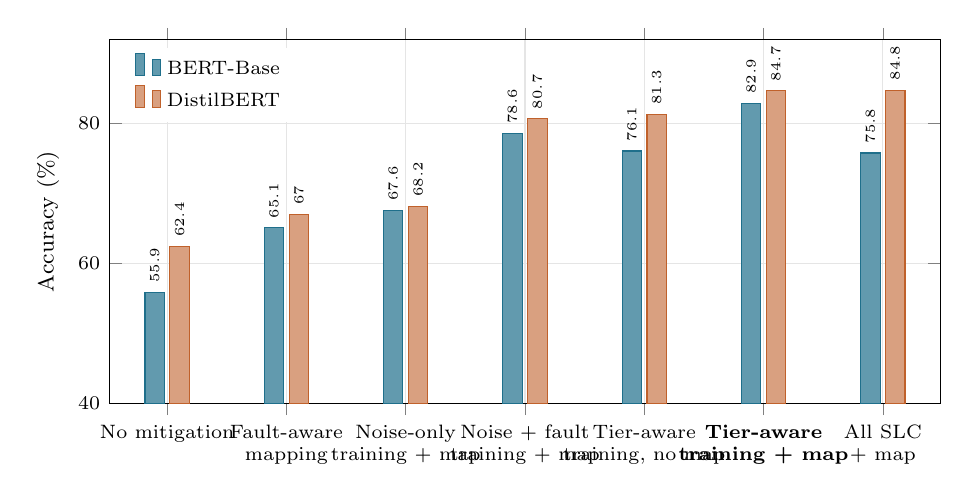
\begin{tikzpicture}
\begin{axis}[ybar,width=\textwidth,height=6.2cm,bar width=7pt,ymin=40,ymax=92,ylabel={Accuracy (\%)},
  symbolic x coords={None,Map,NoiseT,FaultT,TierNoMap,Tier,SLC},xtick=data,
  xticklabels={{No mitigation},{Fault-aware\\mapping},{Noise-only\\training + map},{Noise + fault\\training + map},{Tier-aware\\training, no map},{\textbf{Tier-aware}\\\textbf{training + map}},{All SLC\\+ map}},
  xticklabel style={font=\scriptsize,align=center},tick label style={font=\scriptsize},label style={font=\footnotesize},
  nodes near coords,nodes near coords style={font=\tiny,rotate=90,anchor=west},
  legend style={font=\scriptsize,draw=none,at={(0.02,0.98)},anchor=north west},grid=major,grid style={gray!20},
  enlarge x limits=0.08]
\addplot[fill=cmag!70,draw=cmag] coordinates {(None,55.9) (Map,65.1) (NoiseT,67.6) (FaultT,78.6) (TierNoMap,76.1) (Tier,82.9) (SLC,75.8)};
\addplot[fill=cgrad!60,draw=cgrad] coordinates {(None,62.4) (Map,67.0) (NoiseT,68.2) (FaultT,80.7) (TierNoMap,81.3) (Tier,84.7) (SLC,84.8)};
\legend{BERT-Base,DistilBERT}
\end{axis}
\end{tikzpicture}
\caption{Accuracy at 1\% stuck cells, no programming noise, mean of 10 chips. All bars except the last are the
hybrid chip (magnitude placement, 20\% SLC).}\label{f:bar}
\end{figure}

\begin{table}[H]
\centering\small
\caption{Paired differences of tier-aware training + mapping, in accuracy points (mean $\pm$ s.e., 10 chips).}\label{t:trpaired}
\setlength{\tabcolsep}{3.5pt}
\resizebox{\textwidth}{!}{%
\begin{tabular}{@{}ll cccc ccc cc@{}}
\toprule
& & \multicolumn{4}{c}{Stuck cells, no noise} & \multicolumn{3}{c}{Stuck cells, $\sigma=5\%$} & \multicolumn{2}{c}{1\% stuck} \\
\cmidrule(lr){3-6}\cmidrule(lr){7-9}\cmidrule(l){10-11}
Compared with & Model & 0.2\% & 0.5\% & 1\% & 2\% & 0.2\% & 0.5\% & 1\% & clusters & lines \\
\midrule
\multirow{2}{*}{mapping only} & BERT & $-1.2\pm0.2$ & $+2.7\pm0.5$ & $+17.8\pm2.2$ & $+0.8\pm1.0$ & $+1.6\pm0.5$ & $+7.4\pm0.8$ & $+22.4\pm1.8$ & $+20.7\pm1.6$ & $+20.8\pm2.8$ \\
 & Distil & $-0.1\pm0.2$ & $+3.0\pm0.8$ & $+17.7\pm2.7$ & $+4.1\pm2.4$ & $+0.5\pm0.4$ & $+3.9\pm0.6$ & $+14.7\pm2.4$ & $+14.9\pm2.4$ & $+16.5\pm3.1$ \\
\midrule
\multirow{2}{*}{noise + fault training} & BERT & $-1.0\pm0.2$ & $-0.4\pm0.4$ & $+4.3\pm2.2$ & $+2.2\pm1.0$ & $-0.6\pm0.4$ & $+0.4\pm0.3$ & $+7.5\pm1.8$ & $+6.2\pm1.7$ & $+5.1\pm3.7$ \\
 & Distil & $-0.4\pm0.2$ & $-0.1\pm0.2$ & $+4.0\pm0.6$ & $+2.4\pm1.7$ & $-0.5\pm0.3$ & $+0.5\pm0.3$ & $+2.3\pm1.6$ & $+2.7\pm1.3$ & $+2.8\pm0.8$ \\
\midrule
\multirow{2}{*}{all SLC + mapping} & BERT & $-0.8\pm0.3$ & $+4.6\pm0.7$ & $+7.1\pm3.3$ & $-2.9\pm2.2$ & $+2.9\pm1.4$ & $+5.4\pm1.0$ & $+4.0\pm1.7$ & $+3.7\pm1.4$ & $+0.2\pm3.0$ \\
 & Distil & $+0.3\pm0.2$ & $+0.5\pm0.5$ & $-0.0\pm0.9$ & $-4.9\pm3.1$ & $+0.7\pm0.3$ & $+0.1\pm0.3$ & $-0.9\pm2.4$ & $-2.2\pm1.2$ & $+3.0\pm1.9$ \\
\bottomrule
\end{tabular}}
\end{table}

\begin{table}[H]
\centering\small
\caption{Accuracy (\%) under programming noise alone (no stuck cells), hybrid with 20\% SLC by magnitude,
mean of 10 chips; $\sigma=0$ is an error-free chip.}\label{t:trnoise}
\begin{tabular}{@{}lccc@{\hskip 14pt}ccc@{}}
\toprule
& \multicolumn{3}{c}{BERT-Base} & \multicolumn{3}{c}{DistilBERT} \\
\cmidrule(r){2-4}\cmidrule(l){5-7}
Training & $\sigma=0$ & 5\% & 7.5\% & 0 & 5\% & 7.5\% \\
\midrule
No training & 89.7 & 88.7 & 84.2 & 89.1 & 88.2 & 85.6 \\
Noise-only training & 89.9 & 89.7 & 86.3 & 87.4 & 87.6 & 85.6 \\
Noise + fault training & \textbf{90.9} & \textbf{89.9} & \textbf{88.8} & \textbf{89.9} & \textbf{89.3} & 87.6 \\
Tier-aware training & 89.4 & 89.3 & 88.3 & 87.8 & 88.4 & \textbf{88.0} \\
\bottomrule
\end{tabular}
\end{table}

\noindent\textbf{Analysis.}
\begin{itemize}
\item \textbf{Stuck cells must be injected during training}: noise-only training barely moves the bars of
Fig.~\ref{f:bar}, while adding stuck cells gives the largest single step.
\item \textbf{Knowing the tiers helps where errors are dense}: tier-aware training beats tier-unaware training
at 1\% stuck cells, with programming noise and for clustered faults, ties at 0.5\%, and is slightly behind at
0.2\%, the cost of training on the harsher chip (Table~\ref{t:trnoise}, $\sigma=0$).
\item \textbf{Training and mapping are complementary}: training makes the weights tolerate errors, mapping
keeps sensitive values away from known faults; tier-aware training alone already exceeds mapping alone, and
mapping still adds on top.
\item \textbf{The gap to all-SLC closes} (last block of Table~\ref{t:trpaired}): with tier-aware training and
mapping the hybrid beats all-SLC with mapping on BERT-Base and matches it on DistilBERT up to 1\% stuck cells,
with 34\% fewer cells. At 2\% every configuration fails.
\item Training also improves robustness to programming noise alone (Table~\ref{t:trnoise}).
\end{itemize}

\section*{Step 6: Contribution 4, generalisation to MNLI}
\begin{table}[H]
\centering\small
\caption{MNLI (three classes, chance 33.3\%): paired results, in accuracy points (mean $\pm$ s.e.). Raw
accuracies are in Appendix A.6.}\label{t:mnli}
\begin{tabular}{@{}lcc@{}}
\toprule
& BERT-Base & DistilBERT \\
\midrule
Fisher $-$ magnitude, $\sigma=5\%$, all SLC shares (100 chips) & $-0.2\pm0.2$ & $-0.2\pm0.1$ \\
HyFlexPIM gradient $-$ magnitude, same chips & $-3.4\pm0.4$ & $-0.5\pm0.2$ \\
Fault-aware mapping gain at 0.5\% stuck cells (10 chips) & $+20.1\pm3.0$ & $+18.8\pm3.2$ \\
\bottomrule
\end{tabular}
\end{table}
\noindent Both contributions transfer to the harder task: magnitude again matches Fisher and beats the
gradient on BERT-Base, and mapping recovers about 20 points at 0.5\% stuck cells. MNLI also exposed a
simulator limitation: the single 8-bit scale of the vector between a tier's two crossbars costs up to 11
points even on an error-free chip, so only placements and mappings with the same tier sizes are compared.

\section*{Step 7: Overall comparison with the baseline}
\begin{table}[H]
\centering\small
\caption{Accuracy (\%) of the baseline and of our methods, BERT-Base / DistilBERT. All hybrids keep 20\% of
the components in SLC unless stated. Programming-noise rows use the same 20 chips for all columns; stuck-cell
rows take the baseline from the stuck-cell and fault-pattern sweeps and our methods from the mapping
experiment (10 chips), so those comparisons are not paired.}
\setlength{\tabcolsep}{4pt}
\resizebox{\textwidth}{!}{%
\begin{tabular}{@{}lccccc@{}}
\toprule
Scenario & HyFlexPIM baseline & Magnitude & + fault-aware mapping & + tier-aware training & All SLC + mapping \\
\midrule
$\sigma=7.5\%$, 20\% SLC & 81.2 / 83.1 & \gain{84.1 / 85.2} & -- & -- & 85.7 / 87.4$^{\dagger}$ \\
$\sigma=7.5\%$, 5\% SLC & 67.5 / 78.0 & \gain{79.4 / 80.2} & -- & -- & 85.7 / 87.4$^{\dagger}$ \\
\midrule
0.5\% stuck cells & 71.0 / 74.5 & 76.6 / 77.9 & 85.6 / 85.1 & \gain{88.3 / 88.1} & 83.7 / 87.6 \\
1\% stuck cells & 52.8 / 55.4 & 55.9 / 62.4 & 65.1 / 67.0 & \gain{82.9 / 84.7} & 75.8 / 84.8 \\
1\% stuck, $3\times3$ clusters & 51.5 / 56.4 & 53.7 / 55.9 & 64.3 / 68.5 & \gain{85.0 / 83.4} & 81.3 / 85.6 \\
1\% stuck, bit lines & 51.0 / 52.2 & 50.1 / 54.0 & 56.9 / 68.0 & \gain{77.7 / 84.4} & 77.5 / 81.5 \\
\bottomrule
\end{tabular}}

\smallskip
\raggedright\footnotesize $^{\dagger}$all-SLC without mapping (mapping has no effect without stuck cells).
\end{table}

\noindent\textbf{Findings.}
\begin{itemize}
\item \textbf{Placement}: magnitude ranking matches the Fisher estimate of expected damage and beats the
HyFlexPIM gradient at high noise, by $+2.8\pm0.8$ (BERT-Base) and $+2.2\pm0.3$ points (DistilBERT) at 20\% SLC
and $+11.9\pm1.7$ points at 5\% SLC on BERT-Base, on the same chips.
\item \textbf{Fault-aware mapping}: a zero-hardware reordering that improves the hybrid in every stuck-cell
setting, by up to 13.9 points; choosing the tier per chip adds nothing.
\item \textbf{Tier-aware training}: together with mapping, raises the hybrid at 1\% stuck cells from 52.8\% and
55.4\% (HyFlexPIM baseline) to 82.9\% and 84.7\%, matching or beating an all-SLC chip with mapping up to 1\%
scattered stuck cells while using 34\% fewer cells.
\item \textbf{Generality}: the placement and mapping results hold on MNLI.
\end{itemize}

\clearpage
\section*{Appendix: complete results}
\addcontentsline{toc}{section}{Appendix: complete results}
Every experiment with every placement, both models and every sweep point, generated directly from the
result files of the repository \nolinkurl{github.com/Shivanshmittal023/reliable-reram-crossbar}. Each numbered step
folder (\nolinkurl{<step>}) stores its results as \nolinkurl{<step>/results/<experiment>/<model>/sweep_summary.csv} (mean,
standard deviation and worst chip per point), next to \nolinkurl{sweep.csv} with one row per chip; the source
folder of every section is given below. Accuracy in \%, mean over chips; hybrids keep 20\% of the components
in SLC unless stated.

\subsection*{A.1 Programming noise (5 chips per point)}
\noindent Source: \nolinkurl{02_programming_noise/results/noise/}.
\begin{table}[H]
\centering\footnotesize
\caption{Accuracy against programming noise $\sigma$.}
\resizebox{\ifdim\width>\textwidth\textwidth\else\width\fi}{!}{%
\begin{tabular}{@{}llccccccc@{}}
\toprule
Model & Placement & 0\% & 1\% & 2\% & 3\% & 5\% & 7.5\% & 10\% \\
\midrule
\multirow{6}{*}{BERT-Base} & All SLC & 89.9 & 89.6 & 89.3 & 89.1 & 87.8 & 85.9 & 79.7 \\
 & All MLC & 90.0 & 89.3 & 87.3 & 83.9 & 66.3 & 52.2 & 51.3 \\
 & Random & 90.0 & 90.1 & 89.9 & 87.7 & 78.8 & 58.8 & 49.1 \\
 & HyFlexPIM gradient & 89.8 & 90.4 & 90.2 & 90.0 & 88.0 & 79.3 & 67.7 \\
 & Magnitude (ours) & 89.7 & 89.8 & 89.9 & 90.0 & 88.6 & 83.5 & 72.0 \\
 & Fisher (ours) & 89.1 & 89.7 & 90.1 & 90.0 & 89.0 & 84.5 & 73.7 \\
\midrule
\multirow{6}{*}{DistilBERT} & All SLC & 89.0 & 88.7 & 88.8 & 88.6 & 88.5 & 87.5 & 85.9 \\
 & All MLC & 89.1 & 88.4 & 87.9 & 86.1 & 74.5 & 60.4 & 56.0 \\
 & Random & 88.6 & 88.7 & 88.7 & 87.8 & 82.8 & 61.8 & 52.4 \\
 & HyFlexPIM gradient & 89.8 & 88.5 & 88.9 & 88.7 & 87.7 & 83.4 & 69.8 \\
 & Magnitude (ours) & 89.1 & 88.9 & 88.9 & 88.9 & 88.4 & 85.9 & 77.7 \\
 & Fisher (ours) & 89.0 & 89.0 & 89.0 & 89.1 & 88.5 & 85.5 & 77.6 \\
\bottomrule
\end{tabular}}
\end{table}

\subsection*{A.2 SLC share}
\noindent Source: \nolinkurl{03_slc_share/results/slc_share/}.
\begin{table}[H]
\centering\footnotesize
\caption{BERT-Base: accuracy by share of components in SLC (20 chips per point).}
\begin{tabular}{@{}lcccccccc@{}}
\toprule
$\sigma$ & Placement & 0\% & 5\% & 10\% & 20\% & 30\% & 50\% & 100\% \\
\midrule
\multirow{4}{*}{3\%} & Magnitude (ours) & 82.1 & 89.7 & 89.9 & 89.8 & 89.8 & 89.7 & 89.2 \\
 & Fisher (ours) & 82.1 & 89.6 & 89.8 & 89.8 & 89.8 & 89.8 & 89.2 \\
 & HyFlexPIM gradient & 82.1 & 88.7 & 90.0 & 90.0 & 89.9 & 89.6 & 89.2 \\
 & Random & 82.1 & 87.0 & 86.9 & 87.6 & 87.3 & 89.0 & 89.2 \\
\midrule
\multirow{4}{*}{5\%} & Magnitude (ours) & 66.8 & 88.0 & 88.6 & 88.7 & 88.9 & 88.9 & 88.0 \\
 & Fisher (ours) & 66.8 & 87.9 & 88.6 & 88.8 & 88.9 & 88.9 & 88.0 \\
 & HyFlexPIM gradient & 66.8 & 84.2 & 88.2 & 88.4 & 88.4 & 88.1 & 88.0 \\
 & Random & 66.8 & 72.5 & 73.6 & 76.2 & 77.8 & 83.4 & 88.0 \\
\midrule
\multirow{4}{*}{7.5\%} & Magnitude (ours) & 53.0 & 79.4 & 81.8 & 84.1 & 85.5 & 85.6 & 85.7 \\
 & Fisher (ours) & 53.0 & 80.0 & 82.2 & 84.2 & 85.1 & 85.8 & 85.7 \\
 & HyFlexPIM gradient & 53.0 & 67.5 & 79.0 & 81.2 & 82.4 & 83.2 & 85.7 \\
 & Random & 53.0 & 53.6 & 54.2 & 55.2 & 57.5 & 67.3 & 85.7 \\
\bottomrule
\end{tabular}
\end{table}

\begin{table}[H]
\centering\footnotesize
\caption{DistilBERT: accuracy by share of components in SLC (20 chips per point).}
\begin{tabular}{@{}lcccccccc@{}}
\toprule
$\sigma$ & Placement & 0\% & 5\% & 10\% & 20\% & 30\% & 50\% & 100\% \\
\midrule
\multirow{4}{*}{3\%} & Magnitude (ours) & 86.0 & 88.4 & 88.6 & 88.8 & 88.9 & 88.7 & 88.7 \\
 & Fisher (ours) & 86.0 & 88.5 & 88.7 & 88.7 & 88.8 & 88.6 & 88.7 \\
 & HyFlexPIM gradient & 86.0 & 88.4 & 88.5 & 88.6 & 88.8 & 88.7 & 88.7 \\
 & Random & 86.0 & 86.4 & 86.8 & 87.5 & 88.1 & 88.4 & 88.7 \\
\midrule
\multirow{4}{*}{5\%} & Magnitude (ours) & 74.8 & 87.4 & 88.0 & 88.1 & 88.8 & 88.4 & 88.2 \\
 & Fisher (ours) & 74.8 & 87.3 & 87.8 & 88.4 & 88.1 & 88.3 & 88.2 \\
 & HyFlexPIM gradient & 74.8 & 87.3 & 87.3 & 87.7 & 88.1 & 87.8 & 88.2 \\
 & Random & 74.8 & 75.4 & 77.4 & 81.9 & 82.3 & 85.7 & 88.2 \\
\midrule
\multirow{4}{*}{7.5\%} & Magnitude (ours) & 56.9 & 80.2 & 84.0 & 85.2 & 86.6 & 86.9 & 87.4 \\
 & Fisher (ours) & 56.9 & 80.8 & 83.8 & 85.4 & 86.0 & 87.0 & 87.4 \\
 & HyFlexPIM gradient & 56.9 & 78.0 & 80.7 & 83.1 & 84.8 & 86.0 & 87.4 \\
 & Random & 56.9 & 56.4 & 58.2 & 63.1 & 64.7 & 73.7 & 87.4 \\
\bottomrule
\end{tabular}
\end{table}

\subsection*{A.3 Stuck cells (20 chips per point, no noise)}
\noindent Source: \nolinkurl{04_stuck_cells/results/fault/}.
\begin{table}[H]
\centering\footnotesize
\caption{Accuracy against the share of stuck cells $p$.}
\resizebox{\ifdim\width>\textwidth\textwidth\else\width\fi}{!}{%
\begin{tabular}{@{}llccccccc@{}}
\toprule
Model & Placement & 0\% & 0.1\% & 0.2\% & 0.5\% & 1\% & 2\% & 5\% \\
\midrule
\multirow{6}{*}{BERT-Base} & All SLC & 89.9 & 88.3 & 85.6 & 79.0 & 62.7 & 51.4 & 49.6 \\
 & All MLC & 90.0 & 58.6 & 52.6 & 50.8 & 51.2 & 49.6 & 49.6 \\
 & Random & 90.0 & 67.9 & 55.8 & 50.7 & 50.6 & 50.2 & 49.9 \\
 & HyFlexPIM gradient & 89.8 & 89.4 & 87.5 & 71.0 & 52.8 & 50.2 & 49.5 \\
 & Magnitude (ours) & 89.7 & 89.6 & 88.6 & 76.8 & 57.9 & 51.0 & 50.0 \\
 & Fisher (ours) & 89.1 & 89.7 & 88.4 & 75.6 & 55.5 & 49.5 & 50.3 \\
\midrule
\multirow{6}{*}{DistilBERT} & All SLC & 89.0 & 88.2 & 87.8 & 85.2 & 74.6 & 58.5 & 51.5 \\
 & All MLC & 89.1 & 65.5 & 58.2 & 52.3 & 51.1 & 50.2 & 49.4 \\
 & Random & 88.6 & 76.9 & 63.3 & 51.3 & 51.0 & 49.4 & 50.1 \\
 & HyFlexPIM gradient & 89.8 & 88.1 & 86.7 & 74.5 & 55.4 & 51.0 & 50.5 \\
 & Magnitude (ours) & 89.1 & 88.3 & 87.4 & 80.3 & 62.1 & 51.4 & 49.9 \\
 & Fisher (ours) & 89.0 & 88.3 & 87.2 & 80.3 & 62.1 & 51.3 & 50.4 \\
\bottomrule
\end{tabular}}
\end{table}

\subsection*{A.4 Other non-idealities}
\noindent Source: \nolinkurl{05_other_non_idealities/results/{read,level,cluster,irdrop,adc,adc_noise}/}.
\begin{table}[H]
\centering\footnotesize
\caption{Read noise $\sigma_r$ (5 chips).}
\resizebox{\ifdim\width>\textwidth\textwidth\else\width\fi}{!}{%
\begin{tabular}{@{}llcccccc@{}}
\toprule
Model & Placement & 0\% & 0.5\% & 1\% & 2\% & 3\% & 5\% \\
\midrule
\multirow{5}{*}{BERT-Base} & All SLC & 89.7 & 89.8 & 89.8 & 89.0 & 87.2 & 80.0 \\
 & All MLC & 90.4 & 89.4 & 87.7 & 77.3 & 63.8 & 53.0 \\
 & HyFlexPIM gradient & 90.3 & 90.5 & 90.3 & 89.8 & 88.3 & 76.6 \\
 & Magnitude (ours) & 90.6 & 90.1 & 89.9 & 90.1 & 89.3 & 82.5 \\
 & Fisher (ours) & 89.6 & 90.0 & 89.9 & 89.7 & 89.0 & 82.7 \\
\midrule
\multirow{5}{*}{DistilBERT} & All SLC & 88.5 & 89.0 & 88.2 & 88.3 & 87.5 & 84.5 \\
 & All MLC & 89.0 & 88.6 & 87.9 & 83.8 & 74.5 & 57.7 \\
 & HyFlexPIM gradient & 88.6 & 88.9 & 88.5 & 88.1 & 86.8 & 80.5 \\
 & Magnitude (ours) & 88.8 & 88.9 & 88.7 & 88.4 & 87.7 & 83.3 \\
 & Fisher (ours) & 89.1 & 88.8 & 88.7 & 88.2 & 87.5 & 83.2 \\
\bottomrule
\end{tabular}}
\end{table}

\begin{table}[H]
\centering\footnotesize
\caption{MLC level-dependent noise at $\sigma=5\%$ (10 chips).}
\resizebox{\ifdim\width>\textwidth\textwidth\else\width\fi}{!}{%
\begin{tabular}{@{}llccc@{}}
\toprule
Model & Placement & uniform & mid $\times1.5$ & mid $\times2$ \\
\midrule
\multirow{5}{*}{BERT-Base} & All SLC & 88.2 & 88.2 & 88.2 \\
 & All MLC & 67.3 & 64.7 & 62.5 \\
 & HyFlexPIM gradient & 88.3 & 88.1 & 87.8 \\
 & Magnitude (ours) & 88.9 & 88.7 & 88.4 \\
 & Fisher (ours) & 89.0 & 88.9 & 88.4 \\
\midrule
\multirow{5}{*}{DistilBERT} & All SLC & 88.4 & 88.4 & 88.4 \\
 & All MLC & 75.7 & 73.5 & 70.3 \\
 & HyFlexPIM gradient & 88.0 & 87.5 & 87.1 \\
 & Magnitude (ours) & 88.4 & 88.3 & 88.0 \\
 & Fisher (ours) & 88.1 & 88.0 & 87.9 \\
\bottomrule
\end{tabular}}
\end{table}

\begin{table}[H]
\centering\footnotesize
\caption{Fault patterns at 1\% stuck cells (10 chips).}
\resizebox{\ifdim\width>\textwidth\textwidth\else\width\fi}{!}{%
\begin{tabular}{@{}llccc@{}}
\toprule
Model & Placement & scattered & clusters & lines \\
\midrule
\multirow{5}{*}{BERT-Base} & All SLC & 61.3 & 66.7 & 57.0 \\
 & All MLC & 50.7 & 50.8 & 50.4 \\
 & HyFlexPIM gradient & 52.6 & 51.5 & 51.0 \\
 & Magnitude (ours) & 56.4 & 54.0 & 50.4 \\
 & Fisher (ours) & 55.6 & 53.1 & 52.2 \\
\midrule
\multirow{5}{*}{DistilBERT} & All SLC & 74.2 & 80.3 & 71.2 \\
 & All MLC & 51.2 & 51.2 & 50.8 \\
 & HyFlexPIM gradient & 55.0 & 56.4 & 52.2 \\
 & Magnitude (ours) & 62.5 & 56.1 & 54.7 \\
 & Fisher (ours) & 60.0 & 57.3 & 56.3 \\
\bottomrule
\end{tabular}}
\end{table}

\begin{table}[H]
\centering\footnotesize
\caption{IR drop, wire resistance $r$ (deterministic).}
\resizebox{\ifdim\width>\textwidth\textwidth\else\width\fi}{!}{%
\begin{tabular}{@{}llccccc@{}}
\toprule
Model & Placement & 0 & $10^{-4}$ & $3\times10^{-4}$ & $10^{-3}$ & $3\times10^{-3}$ \\
\midrule
\multirow{5}{*}{BERT-Base} & All SLC & 89.7 & 90.3 & 88.9 & 87.0 & 58.5 \\
 & All MLC & 90.4 & 89.3 & 89.8 & 90.6 & 79.1 \\
 & HyFlexPIM gradient & 90.3 & 90.5 & 90.5 & 88.6 & 76.4 \\
 & Magnitude (ours) & 90.6 & 90.1 & 90.4 & 88.1 & 76.8 \\
 & Fisher (ours) & 89.6 & 91.1 & 91.1 & 88.3 & 72.8 \\
\midrule
\multirow{5}{*}{DistilBERT} & All SLC & 88.5 & 89.9 & 89.4 & 85.3 & 70.1 \\
 & All MLC & 89.0 & 88.6 & 89.1 & 89.9 & 77.9 \\
 & HyFlexPIM gradient & 88.6 & 89.6 & 89.6 & 86.9 & 74.7 \\
 & Magnitude (ours) & 88.8 & 89.2 & 89.7 & 86.6 & 73.4 \\
 & Fisher (ours) & 89.1 & 89.2 & 89.3 & 86.4 & 72.6 \\
\bottomrule
\end{tabular}}
\end{table}

\begin{table}[H]
\centering\footnotesize
\caption{Fixed ADC resolution with bit-serial inputs (deterministic).}
\resizebox{\ifdim\width>\textwidth\textwidth\else\width\fi}{!}{%
\begin{tabular}{@{}llccccccc@{}}
\toprule
Model & Placement & ideal & 8 bit & 7 bit & 6 bit & 5 bit & 4 bit & 3 bit \\
\midrule
\multirow{5}{*}{BERT-Base} & All SLC & 89.7 & 89.9 & 90.0 & 89.3 & 51.1 & 61.1 & 51.1 \\
 & All MLC & 90.4 & 89.6 & 89.2 & 83.0 & 51.1 & 60.3 & 50.9 \\
 & HyFlexPIM gradient & 90.3 & 90.1 & 90.1 & 89.6 & 53.0 & 63.2 & 51.9 \\
 & Magnitude (ours) & 90.6 & 90.4 & 89.3 & 90.0 & 51.1 & 59.9 & 52.6 \\
 & Fisher (ours) & 89.6 & 90.1 & 89.7 & 90.5 & 51.6 & 57.0 & 52.9 \\
\midrule
\multirow{5}{*}{DistilBERT} & All SLC & 88.5 & 89.2 & 88.4 & 88.0 & 71.0 & 52.1 & 59.1 \\
 & All MLC & 89.0 & 88.3 & 87.8 & 81.7 & 56.5 & 51.9 & 56.8 \\
 & HyFlexPIM gradient & 88.6 & 88.4 & 88.5 & 88.4 & 77.3 & 51.5 & 60.1 \\
 & Magnitude (ours) & 88.8 & 88.6 & 89.0 & 89.7 & 70.6 & 51.4 & 62.4 \\
 & Fisher (ours) & 89.1 & 88.0 & 88.2 & 88.8 & 70.9 & 51.7 & 60.3 \\
\bottomrule
\end{tabular}}
\end{table}

\begin{table}[H]
\centering\footnotesize
\caption{Fixed ADC with $\sigma=5\%$ programming noise (3 chips).}
\resizebox{\ifdim\width>\textwidth\textwidth\else\width\fi}{!}{%
\begin{tabular}{@{}llcccc@{}}
\toprule
Model & Placement & ideal & 8 bit & 6 bit & 4 bit \\
\midrule
\multirow{5}{*}{DistilBERT} & All SLC & 88.1 & 88.3 & 88.7 & 52.6 \\
 & All MLC & 77.8 & 76.8 & 56.0 & 53.6 \\
 & HyFlexPIM gradient & 87.8 & 87.6 & 87.2 & 51.8 \\
 & Magnitude (ours) & 88.7 & 89.1 & 88.5 & 51.5 \\
 & Fisher (ours) & 87.8 & 88.5 & 88.2 & 52.3 \\
\bottomrule
\end{tabular}}
\end{table}

\subsection*{A.5 Fault-aware mapping (10 chips per point)}
\noindent Source: \nolinkurl{06_fault_aware_mapping/results/{fault,fault_noise,pattern}/}.
\begin{table}[H]
\centering\footnotesize
\caption{Stuck cells, no noise.}
\resizebox{\ifdim\width>\textwidth\textwidth\else\width\fi}{!}{%
\begin{tabular}{@{}llcccc@{}}
\toprule
Model & Placement & 0.2\% & 0.5\% & 1\% & 2\% \\
\midrule
\multirow{5}{*}{BERT-Base} & All SLC & 85.4 & 80.1 & 60.9 & 51.1 \\
 & All SLC + fault-aware mapping & 89.6 & 83.7 & 75.8 & 55.9 \\
 & Hybrid, no mitigation & 88.5 & 76.6 & 55.9 & 50.1 \\
 & Hybrid + fault-aware mapping & 90.1 & 85.6 & 65.1 & 52.2 \\
 & Hybrid + joint mapping & 90.0 & 84.3 & 68.3 & 49.4 \\
\midrule
\multirow{5}{*}{DistilBERT} & All SLC & 88.1 & 85.4 & 73.7 & 57.9 \\
 & All SLC + fault-aware mapping & 88.0 & 87.6 & 84.8 & 62.3 \\
 & Hybrid, no mitigation & 87.1 & 77.9 & 62.4 & 50.2 \\
 & Hybrid + fault-aware mapping & 88.4 & 85.1 & 67.0 & 53.3 \\
 & Hybrid + joint mapping & 88.3 & 85.3 & 67.7 & 54.7 \\
\bottomrule
\end{tabular}}
\end{table}

\begin{table}[H]
\centering\footnotesize
\caption{Stuck cells with $\sigma=5\%$.}
\resizebox{\ifdim\width>\textwidth\textwidth\else\width\fi}{!}{%
\begin{tabular}{@{}llccc@{}}
\toprule
Model & Placement & 0.2\% & 0.5\% & 1\% \\
\midrule
\multirow{5}{*}{BERT-Base} & All SLC & 85.6 & 78.4 & 64.6 \\
 & All SLC + fault-aware mapping & 86.1 & 82.4 & 76.5 \\
 & Hybrid, no mitigation & 84.9 & 70.3 & 52.1 \\
 & Hybrid + fault-aware mapping & 87.4 & 80.4 & 58.1 \\
 & Hybrid + joint mapping & 87.2 & 77.9 & 61.7 \\
\midrule
\multirow{5}{*}{DistilBERT} & All SLC & 86.9 & 81.7 & 68.0 \\
 & All SLC + fault-aware mapping & 87.6 & 86.8 & 80.7 \\
 & Hybrid, no mitigation & 85.4 & 74.9 & 59.5 \\
 & Hybrid + fault-aware mapping & 87.7 & 83.0 & 65.1 \\
 & Hybrid + joint mapping & 87.0 & 82.3 & 63.1 \\
\bottomrule
\end{tabular}}
\end{table}

\begin{table}[H]
\centering\footnotesize
\caption{1\% stuck cells by pattern.}
\resizebox{\ifdim\width>\textwidth\textwidth\else\width\fi}{!}{%
\begin{tabular}{@{}llcc@{}}
\toprule
Model & Placement & clusters & lines \\
\midrule
\multirow{5}{*}{BERT-Base} & All SLC & 66.5 & 57.2 \\
 & All SLC + fault-aware mapping & 81.3 & 77.5 \\
 & Hybrid, no mitigation & 53.7 & 50.1 \\
 & Hybrid + fault-aware mapping & 64.3 & 56.9 \\
 & Hybrid + joint mapping & 61.5 & 56.8 \\
\midrule
\multirow{5}{*}{DistilBERT} & All SLC & 79.6 & 71.1 \\
 & All SLC + fault-aware mapping & 85.6 & 81.5 \\
 & Hybrid, no mitigation & 55.9 & 54.0 \\
 & Hybrid + fault-aware mapping & 68.5 & 68.0 \\
 & Hybrid + joint mapping & 75.5 & 62.7 \\
\bottomrule
\end{tabular}}
\end{table}

\subsection*{A.6 MNLI (2{,}000 matched validation pairs)}
\noindent Source: \nolinkurl{08_mnli/results/{slc_share,fault,mapping}/}.
\begin{table}[H]
\centering\footnotesize
\caption{MNLI: accuracy by share of components in SLC at $\sigma=5\%$ (20 chips per point).}
\begin{tabular}{@{}llccccccc@{}}
\toprule
Model & Placement & 0\% & 5\% & 10\% & 20\% & 30\% & 50\% & 100\% \\
\midrule
\multirow{4}{*}{BERT-Base} & Magnitude (ours) & 33.5 & 64.0 & 66.0 & 68.0 & 69.2 & 66.7 & 61.6 \\
 & Fisher (ours) & 33.5 & 64.2 & 65.8 & 67.8 & 68.8 & 66.6 & 61.6 \\
 & HyFlexPIM gradient & 33.5 & 59.6 & 63.5 & 63.3 & 66.5 & 64.2 & 61.6 \\
 & Random & 33.5 & 34.1 & 33.9 & 35.9 & 38.9 & 44.9 & 61.6 \\
\midrule
\multirow{4}{*}{DistilBERT} & Magnitude (ours) & 36.8 & 68.4 & 70.0 & 71.5 & 72.6 & 72.5 & 72.0 \\
 & Fisher (ours) & 36.8 & 68.5 & 70.0 & 71.1 & 72.1 & 72.3 & 72.0 \\
 & HyFlexPIM gradient & 36.8 & 66.6 & 69.0 & 71.3 & 72.1 & 73.6 & 72.0 \\
 & Random & 36.8 & 38.3 & 39.3 & 44.1 & 48.1 & 55.3 & 72.0 \\
\bottomrule
\end{tabular}
\end{table}

\begin{table}[H]
\centering\footnotesize
\caption{MNLI: stuck cells, 20\% SLC (20 chips).}
\resizebox{\ifdim\width>\textwidth\textwidth\else\width\fi}{!}{%
\begin{tabular}{@{}llccccccc@{}}
\toprule
Model & Placement & 0\% & 0.1\% & 0.2\% & 0.5\% & 1\% & 2\% & 5\% \\
\midrule
\multirow{6}{*}{BERT-Base} & All SLC & 72.2 & 67.2 & 61.9 & 44.4 & 34.5 & 32.4 & 32.4 \\
 & All MLC & 72.4 & 37.2 & 33.2 & 32.8 & 31.8 & 31.9 & 32.3 \\
 & Random & 73.0 & 42.8 & 34.3 & 33.3 & 32.6 & 32.4 & 33.5 \\
 & HyFlexPIM gradient & 78.2 & 73.0 & 65.2 & 36.9 & 32.0 & 31.5 & 32.4 \\
 & Magnitude (ours) & 79.1 & 74.6 & 67.8 & 40.4 & 32.8 & 32.2 & 32.3 \\
 & Fisher (ours) & 79.3 & 73.9 & 67.2 & 39.8 & 32.8 & 32.3 & 32.6 \\
\midrule
\multirow{6}{*}{DistilBERT} & All SLC & 76.9 & 74.4 & 71.3 & 60.4 & 42.1 & 34.1 & 34.2 \\
 & All MLC & 76.8 & 44.5 & 34.0 & 33.6 & 33.7 & 34.1 & 33.0 \\
 & Random & 77.7 & 51.6 & 35.3 & 32.9 & 33.2 & 33.7 & 33.4 \\
 & HyFlexPIM gradient & 79.6 & 76.0 & 71.4 & 44.5 & 33.9 & 32.9 & 33.9 \\
 & Magnitude (ours) & 77.3 & 74.8 & 71.3 & 49.7 & 34.0 & 33.3 & 33.8 \\
 & Fisher (ours) & 78.3 & 74.9 & 70.7 & 50.3 & 34.0 & 33.6 & 33.1 \\
\bottomrule
\end{tabular}}
\end{table}

\begin{table}[H]
\centering\footnotesize
\caption{MNLI: fault-aware mapping (10 chips).}
\resizebox{\ifdim\width>\textwidth\textwidth\else\width\fi}{!}{%
\begin{tabular}{@{}llcccc@{}}
\toprule
Model & Placement & 0.2\% & 0.5\% & 1\% & 2\% \\
\midrule
\multirow{5}{*}{BERT-Base} & All SLC & 61.5 & 46.7 & 35.7 & 33.2 \\
 & All SLC + fault-aware mapping & 69.9 & 61.9 & 46.2 & 33.1 \\
 & Hybrid, no mitigation & 68.1 & 40.0 & 33.1 & 32.2 \\
 & Hybrid + fault-aware mapping & 75.3 & 60.0 & 36.5 & 32.3 \\
 & Hybrid + joint mapping & 75.5 & 60.4 & 35.5 & 32.3 \\
\midrule
\multirow{5}{*}{DistilBERT} & All SLC & 71.4 & 58.4 & 41.4 & 34.6 \\
 & All SLC + fault-aware mapping & 76.2 & 72.2 & 58.5 & 37.4 \\
 & Hybrid, no mitigation & 69.9 & 49.1 & 33.4 & 33.4 \\
 & Hybrid + fault-aware mapping & 76.6 & 67.9 & 38.8 & 34.3 \\
 & Hybrid + joint mapping & 76.6 & 67.0 & 39.4 & 33.3 \\
\bottomrule
\end{tabular}}
\end{table}

\subsection*{A.7 Training: every variant with and without fault-aware mapping (10 chips per point)}
\noindent Source: \nolinkurl{07_training/results/<variant>/<experiment>/}, with variants \nolinkurl{nat_noise},
\nolinkurl{nat_fault} and \nolinkurl{tier_aware}, and experiments \nolinkurl{fault}, \nolinkurl{fault_noise} and \nolinkurl{pattern}.
\begin{table}[H]
\centering\footnotesize
\caption{Accuracy (\%) of the hybrid chip (20\% SLC by magnitude) for each training variant, without and with fault-aware mapping. The untrained model is in A.5.}
\resizebox{\textwidth}{!}{%
\begin{tabular}{@{}lll cccc ccc cc@{}}
\toprule
& & & \multicolumn{4}{c}{Stuck cells, no noise} & \multicolumn{3}{c}{Stuck cells, $\sigma=5\%$} & \multicolumn{2}{c}{1\% stuck} \\
\cmidrule(lr){4-7}\cmidrule(lr){8-10}\cmidrule(l){11-12}
Model & Training & Mapping & 0.2\% & 0.5\% & 1\% & 2\% & 0.2\% & 0.5\% & 1\% & clusters & lines \\
\midrule
\multirow{6}{*}{BERT-Base}  & \multirow{2}{*}{Noise only} & no & 89.3 & 80.6 & 56.9 & 51.0 & 87.1 & 74.1 & 52.9 & 54.4 & 50.1 \\
 &  & yes & 89.8 & 87.0 & 67.6 & 51.7 & 88.0 & 82.7 & 58.0 & 65.8 & 58.9 \\
 & \multirow{2}{*}{Noise + faults} & no & 89.9 & 87.5 & 66.3 & 50.3 & 88.6 & 83.7 & 60.2 & 58.0 & 52.2 \\
 &  & yes & 89.9 & 88.7 & 78.6 & 50.8 & 89.7 & 87.4 & 72.9 & 78.8 & 72.6 \\
 & \multirow{2}{*}{Tier-aware} & no & 89.2 & 87.1 & 76.1 & 50.8 & 88.6 & 86.5 & 70.0 & 71.3 & 53.1 \\
 &  & yes & 88.8 & 88.3 & 82.9 & 53.0 & 89.1 & 87.8 & 80.5 & 85.0 & 77.7 \\
\midrule
\multirow{6}{*}{DistilBERT}  & \multirow{2}{*}{Noise only} & no & 86.3 & 77.5 & 62.1 & 50.5 & 85.3 & 76.4 & 60.6 & 56.6 & 53.6 \\
 &  & yes & 87.3 & 84.5 & 68.2 & 51.5 & 85.9 & 82.8 & 59.9 & 66.1 & 65.9 \\
 & \multirow{2}{*}{Noise + faults} & no & 88.6 & 83.4 & 72.5 & 50.8 & 88.1 & 83.9 & 67.7 & 68.0 & 57.6 \\
 &  & yes & 88.6 & 88.2 & 80.7 & 55.0 & 88.8 & 86.4 & 77.5 & 80.7 & 81.6 \\
 & \multirow{2}{*}{Tier-aware} & no & 88.2 & 85.7 & 81.2 & 52.9 & 88.1 & 85.6 & 76.5 & 77.7 & 67.5 \\
 &  & yes & 88.2 & 88.1 & 84.7 & 57.4 & 88.2 & 86.9 & 79.8 & 83.4 & 84.4 \\
\bottomrule
\end{tabular}}
\end{table}

The training results under programming noise alone are in Table~\ref{t:trnoise} (Step 5).


\end{document}
